\documentclass[11pt,a4paper]{article}
\usepackage[utf8]{inputenc}
\usepackage[fleqn]{amsmath}
\usepackage{amsfonts}
\usepackage{amssymb}
\usepackage{graphicx}
\usepackage{float}
\usepackage{natbib}
\usepackage{url}
\usepackage[top=1in, bottom=1.25in, left=1.5in, right=1.5in]{geometry}
\usepackage{titlesec}

\begin{document}
	
%%Title Page
\begin{titlepage}
\title{An interactive ray tracing system
\\based on Nvidia OptiX}
\date{01.04.2015 - 30.09.2015}
\author{Michael Größler	 Martin Zettwitz}
\maketitle

\begin{center}

\includegraphics[width=0.7\linewidth]{./OVGU}
\end{center}




\end{titlepage}

\tableofcontents


\newpage
\section{Introduction}
\label{sec:Introduction}
Ray Tracing is an integral part of production rendering and as such much research was devoted to it. As many lighting techniques rely on a robust ray tracing implementation, several middleware packages were shipped for the market. Among those is Nvidia's Ray Tracing Engine OptiX.

The task of our software project can be split into two parts. The first One is to familiarize with this library and other utilities to build an interactive ray tracing application. This requires features such as a content pipeline, basic illumination algorithms like direct lighting and shadowing, modelling and parsing test scenes.

Second, to be able to capture more realistic scenes, the need for physically-based rendering grows. Therefore, several BRDFs(bi-directional distribution function) have had to be implemented and had to be checked for plausibility.

\newpage
\section{System}
\label{sec:System}
In this section we will describe the technical sight on our project. We decided to develop on Linux-based systems to avoid problems due to the integration of libraries, using the better ressource manager, develop on a reliable system and to use fully open source software. Therefore we have chosen Ubuntu 14.04 LTS, not at least because of the good community support. As mentioned above, we used the Nvidia Optix SDK 3.8.0 based on CUDA 7.5 as our basic ray tracing software. OptiX is written in C and CUDA to be a high performant system that distributes the large amount of computations on the high number of GPU cores, since the GPU is perfectly made for the task of parallel computations. The main advantages of the SDK are a given basic system/interface and the most important a link to the GPU, so that we don't have to worry about GPU memory and thread distributions. The OptiX SDK was delivered as a platform independent CMake project, so we had to integrate our libraries and own files into CMake, too. 
Due to a recommendation we used the library "AntTweakBar" as an easy to use GUI to control the parameters of our BRDFs, light and geometry. We used GLUT to connect OptiX to OpenGL.


\newpage
\section{Managing the project}
\label{sec:management}
To handle the large amount of arrangements, meetings, code exchanges, version controlling and other project based tasks we had to plan the whole project from the beginning. First we registered us at the official Nvidia developer page to get access to the Nvidia OptiX SDK and especially to the OptiX documentation. With the basic knowledge about the SDK we started to gather ideas for our project and created a first Gantt chart using the open source software "GanttProject". Several milestones splitted our project into work packages with smaller tasks we could work off parallel. We planned to start implementing the basic ray tracing system, go on with a simple setup like the One from the seminar "Graphik I" of the second semester, create a useful GUI using AntTweakBar, implement a mesh loader and last advanced BRDFs. Basically Michael was more responsible for the setup of the ray tracing engine and Martin for the interface and the interaction between the materials(BRDFs), both of us implemented the BRDFs and helped each other solving bugs. Meetings with our advisor Tobias Günther were planned in a two weeks stroke, so that we were more independet from weeks with more work in the regular university seminars. To exchange code, track issues and develop on tasks, save and independent from the main project, we used the Github with an academical license as our git server. With Github it was easy to see new commits at the first sight, track issues and create tickets for bugs or open tasks and we had a version control system to work independent from other tasks to keep code clean and stable.


\newpage
\section{The Rendering Equation}
\label{sec:renderingequation}
To describe the radiance at point x in space with incoming direction $\vec{\omega_o}$ and incoming light direction $\vec{\omega_i}$, the following equation\cite{Kaj86} is used:

\begin{equation}
L_o(x,\vec{\omega_o}) = L_e(x,\vec{\omega_o}) + \int_\Omega f_r(\vec{\omega_i},\vec{\omega_o}) \cdot \cos\theta \cdot L_i(x,\vec{\omega_i}) \cdot d\vec{\omega_i}\
\label{eq:renderingequation}
\end{equation}

\begin{table}[h]
\begin{tabular}{| c | l |}
\hline
$L_o$ & out-going radiance\\ \hline
$L_e$ & self emission\\ \hline
$L_i$ & in-going radiance\\ \hline
$\vec{\omega_i}$ & incoming light direction\\ \hline
$\vec{\omega_o}$ & vector towards camera\\ \hline
$f_r$ & BRDF\\ \hline
$\Omega$ & Hemisphere over point x\\ \hline
$\cos\theta$ & angle between normal and $\vec{\omega_i}$\\ \hline
$x$ & point on surface\\ \hline
\end{tabular}
\end{table}

In short, to evaluate the radiance of one point in space, one has to sum up the incident light over the hemisphere at this point and his self emission. This includes indirect lighting, which is not implemented, yet.

		
In our approach only direct lighting, reflections and no self emissions are calculated, so we altered the original equation, like the CG raytracer, to the following:

\begin{equation}
L_o(x,\vec{\omega_o}) = \delta L_i(x,\vec{\omega_r}) + (1- \delta) \sum_{i=1}^{k} f_r(\vec{\omega_i},\vec{\omega_o}) \cdot E
\label{eq:simplerenderingequation}
\end{equation}


\begin{table}[H]
\begin{tabular}{| c | l |}
\hline
$\delta$ & reflection coefficient\\ \hline
$E$ & approximated irradiance\\ \hline
$I_o$ & light intensity of a point light (independent from $\vec{\omega_i}$)\\ \hline
\end{tabular}
\end{table}

\begin{equation}
E \approx \frac{I_o \cdot cos\theta}{distance(x,x_L)^2}
\end{equation}


To compute the illumination of a given point, we have to calculate the BRDF for every incoming radiance.

BRDFs are used to describe the behaviour of a surfaces depending on light and view direction.
In the following section we describe our implemented BRDFs, our experience playing around with them and provide pictures to prove their plausibility.


\newpage
\section{BRDFs}
Our BRDFs are composed of two components:
\begin{equation}
f_r = K_d + K_s
\end{equation}
\begin{table}[H]
\begin{tabular}{| c | l |}
\hline
$K_d$ & diffuse component\\ \hline
$K_s$ & specular component\\ \hline
\end{tabular}
\end{table}

Both $K_d$ and $K_s$ will be described for each BRDF we used in our project.

Following terms will be used:
\begin{table}[H]
\begin{tabular}{| c | l |}
\hline
$\vec{V}$ & ray from hit point to camera\\ \hline
$\vec{N}$ & normal on hit point\\ \hline
$\vec{L}$ & ray from hit point to light source\\ \hline
\end{tabular}
\end{table}



\subsection{Lambert}
Based on Lambert's emission law published in 'Photometria' by Johann Heinrich Lambert in 1760. Simulates a perfectly diffuse surface.

\begin{equation}
K_d = \frac{1}{\pi}
\end{equation}
\begin{equation}
K_s = 0
\end{equation}
\\Lambert is a very basic and simple material. Nevertheless it is useful for very matte surfaces like paper. 


\newpage
\subsection{Phong}
Based on \cite{Pho75}. This empirical model is a simple to compute standard model for shiny surfaces and was the first description for non-Lambertian surfaces.

\begin{equation}
K_d = \frac{\rho_d}{\pi}
\end{equation}
\begin{equation}
K_s = \rho_s \cdot \frac{s+2}{2\pi} \cdot cos^s\psi
\end{equation}

\begin{table}[H]
\begin{tabular}{| c | l |}
\hline
$\rho_d$ & Parameter : diffuse coefficient\\ \hline
$\rho_s$ & Parameter : specular coefficient\\ \hline
$s$ & Parameter : shiny exponent, controls roughness\\ \hline
$cos\psi$ & angle between outgoing and reflected ray\\ \hline
\end{tabular}
\end{table}


\begin{figure}[H]
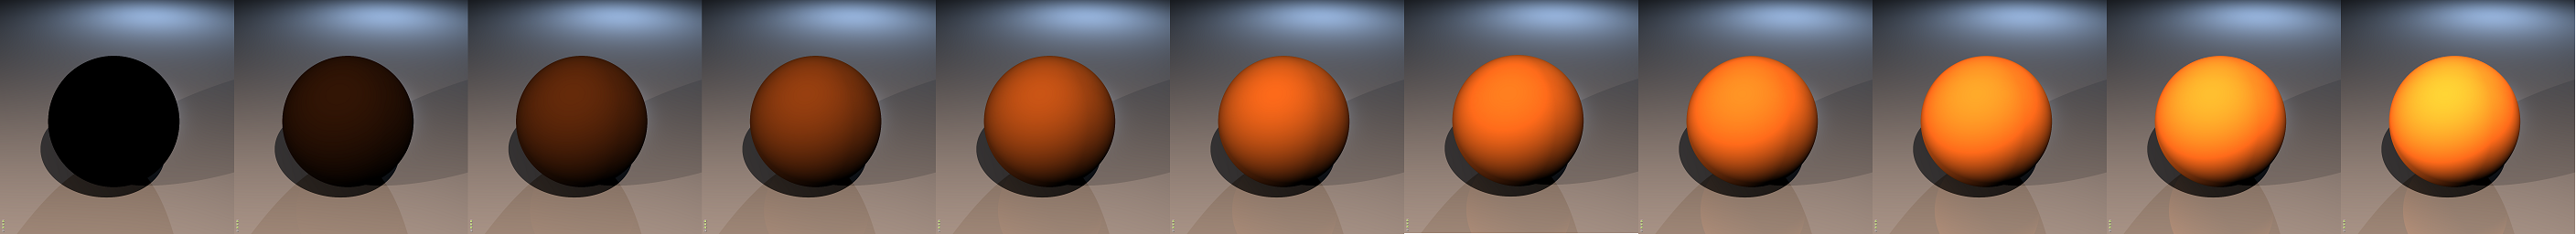
\includegraphics[width=\textwidth]{phongdiffcomplete.png}
\caption{Parameter $\rho_d$ from $0.0$ to $1.0$}
\end{figure}

\begin{figure}[H]
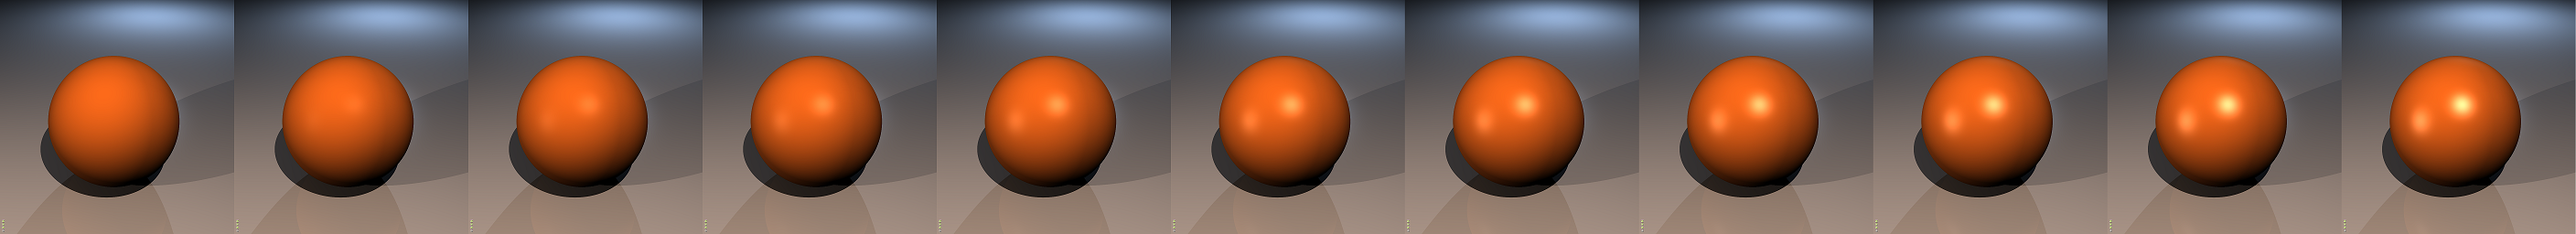
\includegraphics[width=\textwidth]{phongspeccomplete.png}
\caption{Parameter $\rho_s$ from $0.0$ to $1.0$}
\end{figure}

\begin{figure}[H]
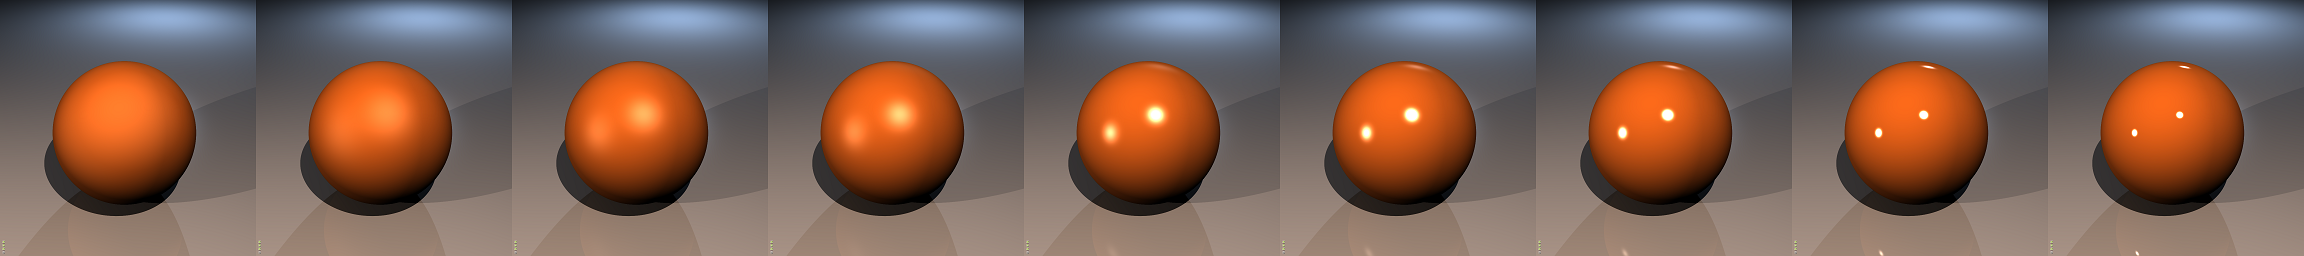
\includegraphics[width=\textwidth]{phongshinecomplete.png}
\caption{Parameter $s$ from $1$ to $1000$}
\end{figure}

\begin{figure}[H]
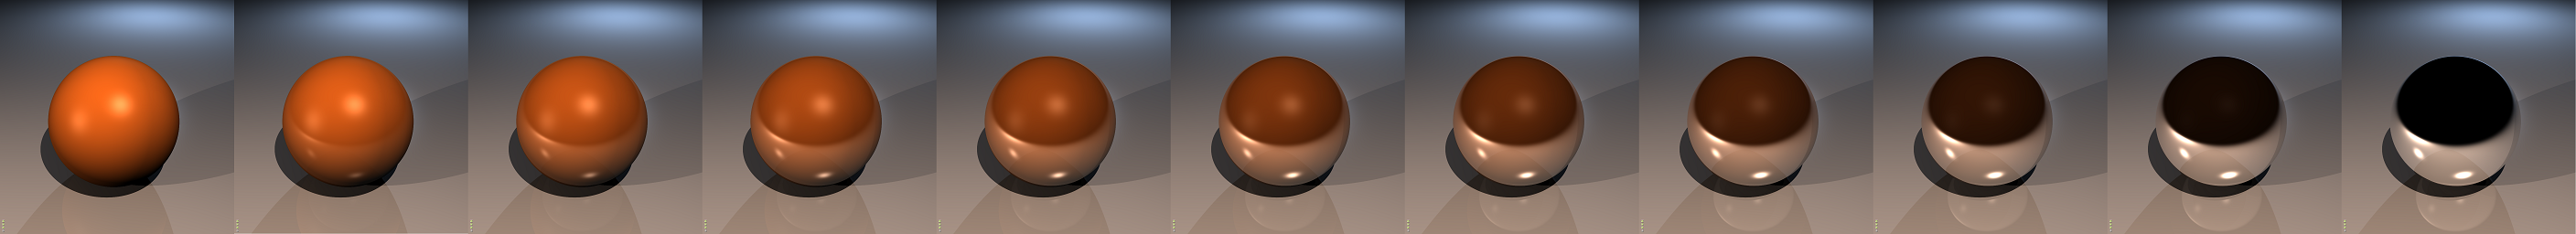
\includegraphics[width=\textwidth]{phongreflcomplete.png}
\caption{Parameter $\delta$(see equation \ref{eq:simplerenderingequation}) from $0.0$ to $1.0$}
\end{figure}


\newpage
\subsection{Blinn Phong}
Based on \cite{Bli77}. The standard Phong model was altered by using the half vector $\vec{H}$. It's the standard lighting model in DirectX and OpenGL.

\begin{equation}
K_d = \frac{\rho_d}{\pi}
\end{equation}
\begin{equation}
K_s = \rho_s \cdot \frac{s+8}{8\pi} \cdot cos^s\psi
\end{equation}

\begin{table}[H]
\begin{tabular}{| c | l |}
\hline
$\cos\psi$ & angle between outgoing ray and half vector $\vec{H}$\\ \hline
\end{tabular}
\end{table}
\begin{equation}
\vec{H} = \frac{\vec{L}+\vec{V}}{length(\vec{L}+\vec{V})}
\label{eq:H}
\end{equation}

\begin{figure}[H]
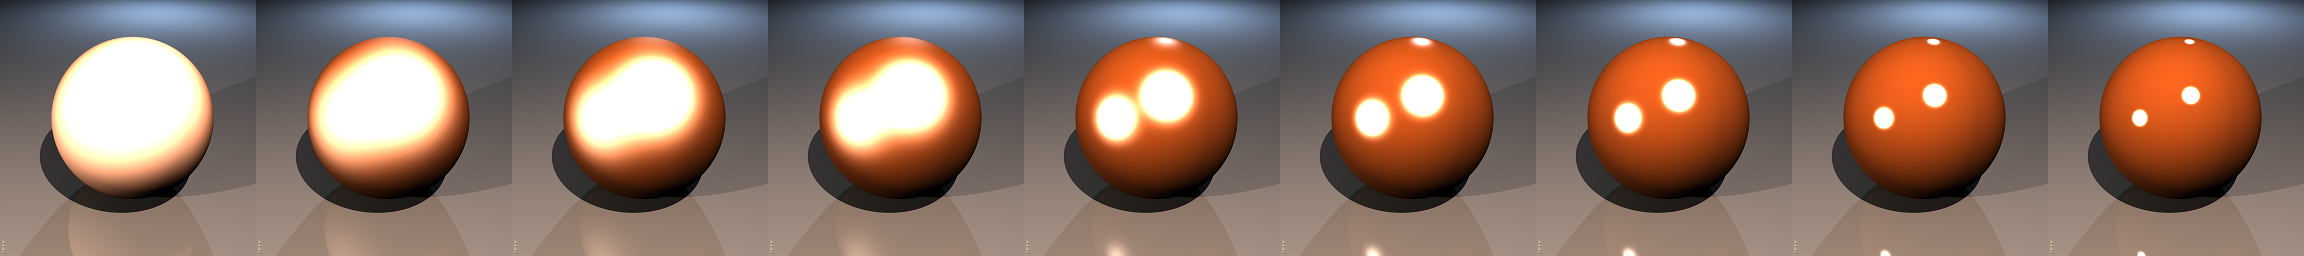
\includegraphics[width=\textwidth]{blinnphongshinecomplete.png}
\caption{Parameter $s$ from $1$ to $1000$}
\end{figure}


\newpage
\subsection{Cook Torrance}
Based on \cite{CT82}. A physically based reflection model using microfacets to simulate isotropic metallic surfaces.
\begin{equation}
K_d = \frac{\rho_d}{\pi}
\end{equation}
\begin{equation}
K_s =\rho_s \frac{D \cdot F \cdot G}{4(\vec{V} \cdot \vec{N})(\vec{N} \cdot \vec{L})}
\end{equation}

\begin{table}[H]
\begin{tabular}{| c | l |}
\hline
$D$ & Beckmann distribution\\ \hline
$F$ & Fresnel term\\ \hline
$G$ & Geometric attenuation (Torrance Sparrow)\\ \hline
\end{tabular}
\end{table}
Beckmann distribution:
\begin{equation}
D = \frac{e^{-\frac{tan^2(\alpha)}{m^2}}}{\pi \cdot m^2 \cdot cos^4(\alpha)}
\label{eq:beckmann}
\\
\alpha = arccos(\vec{N} \cdot \vec{H})
\end{equation}

Fresnel term, based on \cite{Sch94}:
\begin{equation}
F = \delta + (1-\delta)(1-cos(\theta))^5 \\ \delta = \left(\frac{\eta - 1}{\eta+1}\right)^2
\end{equation}


Geometric attenuation:
\begin{equation}
G = min \left(1,\frac{2(\vec{H} \cdot \vec{N})(\vec{V} \cdot \vec{N})}{\vec{V} \cdot \vec{H}},\frac{2 (\vec{H} \cdot \vec{N})(\vec{L} \cdot \vec{N})}{\vec{V} \cdot \vec{H}}\right)
\end{equation}

\begin{table}[H]
\begin{tabular}{| c | l |}
\hline
$m$ & Parameter : controls roughness of surface\\ \hline
$\eta$  & Parameter : Fresnel factor(refractive index)\\ \hline
$\theta$  & Angle between $\vec{l}$ and $\vec{H}$\\ \hline
\end{tabular}
\end{table}
To simplify equation \ref{eq:beckmann}, the following substitution is used:
\begin{equation}
\frac{tan^2(\alpha)}{m^2} = \frac{1- cos^2(\alpha)}{cos^2(\alpha) \cdot m^2}
\end{equation}

\begin{figure}[H]
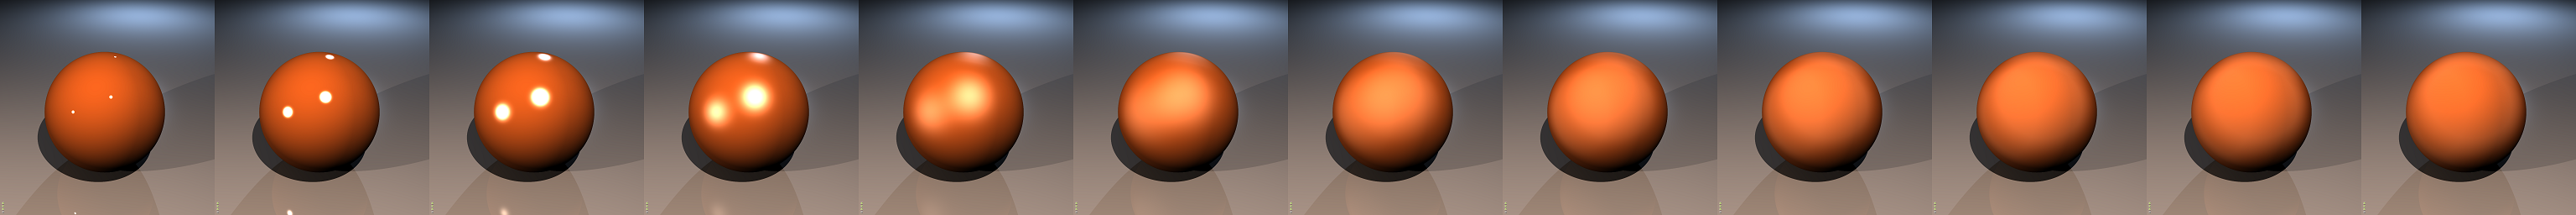
\includegraphics[width=\textwidth]{ctroughcomplete.png}
\caption{Parameter $m$ from $0.01$ to $1.0$}
\end{figure}

\begin{figure}[H]
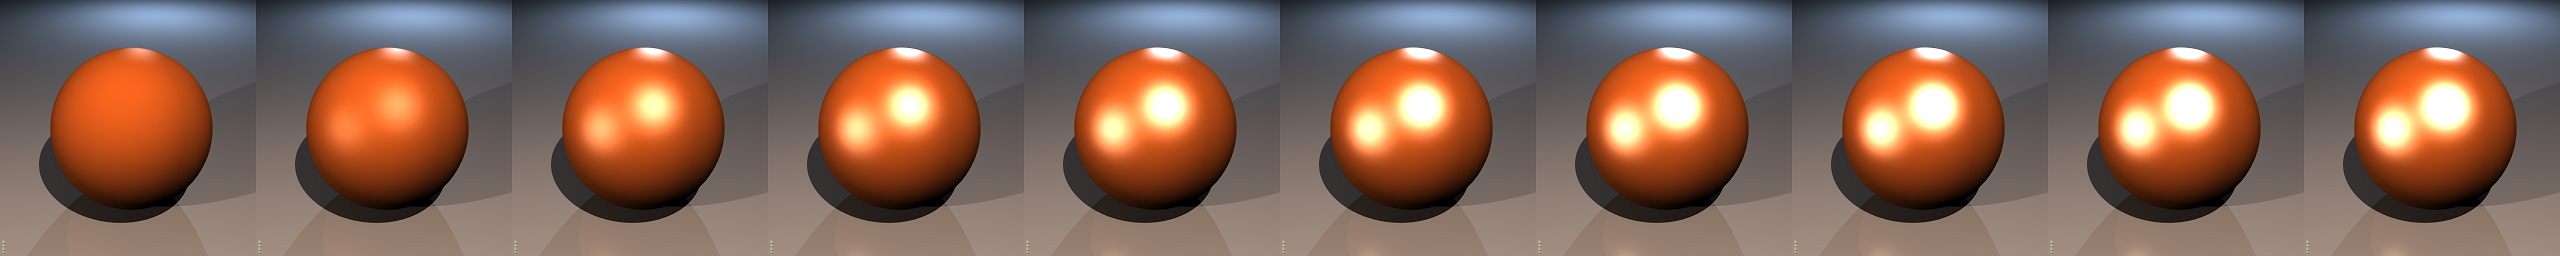
\includegraphics[width=\textwidth]{ctfresnelcomplete.png}
\caption{Parameter $\eta$ from $1.0$ to $10.0$}
\end{figure}


\newpage
\subsection{Ward}
Based on \cite{GMD10}. This is a cheap to compute, mathematical description for anisotropic metallic surfaces. This version expands [War92] by a special normalization term. 

\begin{equation}
K_d = \frac{\rho_d}{\pi}
\end{equation}

\begin{equation}
K_s = \frac{\rho_s}{4 \pi \alpha_x \alpha_y } 
\cdot e^
{
- \frac{(\frac{\vec{h} \cdot \vec{x}}{\alpha_x})+(\frac{\vec{h} \cdot \vec{y}}{\alpha_y})}
{(\vec{h} \cdot \vec{N})^2}
}
\cdot 
\frac{1}{4 (\vec{H} \cdot \vec{L})^2 (\vec{H} \cdot \vec{N})^4}
\end{equation}

\begin{table}[H]
\begin{tabular}{| c | l |}
\hline
$\alpha_x$ & Parameter : horizontal control of brush\\ \hline
$\alpha_y$ & Parameter : vertical control of brush \\ \hline
$\vec{h}$ & Half vector between $\vec{L}$ and $\vec{V}$ \\ \hline
$\vec{H}$ & Normalized half vector between $\vec{L}$ and $\vec{V}$ \\ \hline
$\vec{x}$ & Tangent Vector to $\vec{N}$ \\ \hline
$\vec{y}$ & Tangent Vector to $\vec{N}$, perpendicular to $\vec{x}$ \\ \hline
\end{tabular}
\end{table}

\begin{figure}[H]
\centering

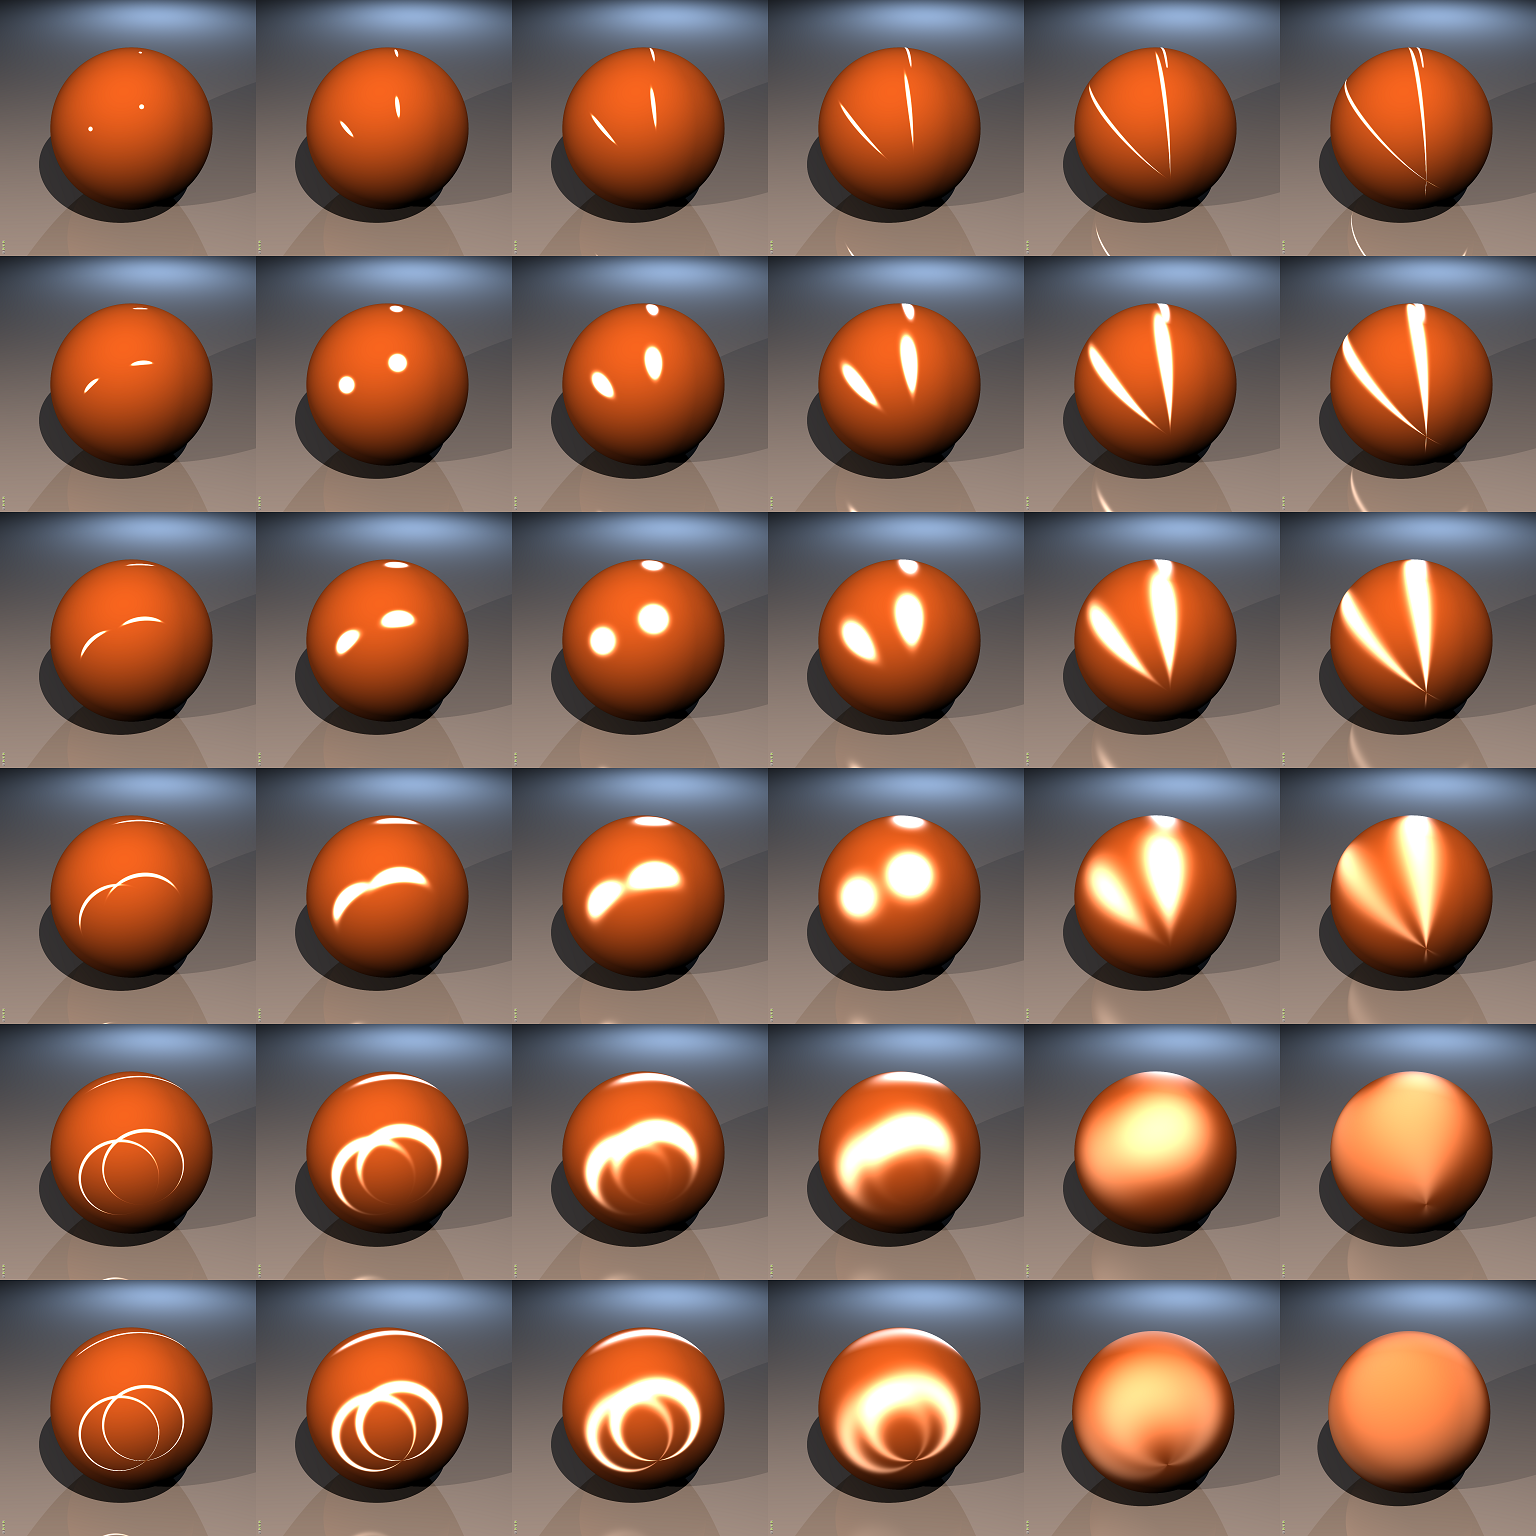
\includegraphics[scale=0.25]{warduvcomplete.png}
\caption{Parameter $\alpha_x$, $\alpha_y$ from $0.01$ to $1.00$}
\end{figure}

\newpage
\subsection{Ashikhmin Shirley}
Based on \cite{AS00}. This model is based on ansioptropic microfacets and is also used for anisotropic metallic surfaces.

\begin{equation}
K_d = \frac{28 \rho_d}{23 \rho_s} (1 - \rho_s)\left(1-\left(1- \frac{\vec{N} \cdot \vec{L}}{2}\right)^5\right)\left(1-\left(1-\frac{\vec{N} \cdot \vec{L}}{2}\right)^5\right)
\end{equation}

\begin{equation}
K_s = \frac{\sqrt{(n_u+1)(n_v+1)}}{8\pi} \frac{((\vec{N} \cdot \vec{H})^{ \frac{n_u(\vec{H} \cdot \vec{U})^2 + n_v(\vec{H} \cdot \vec{V})^2}{1-(\vec{H} \cdot \vec{N})^2})}}{(\vec{H} \cdot \vec{L}) max((\vec{N} \cdot \vec{L}),(\vec{N} \cdot \vec{V}))} F(\vec{L} \cdot \vec{H})
\end{equation}

where:
\begin{equation}
F(\vec{L} \cdot \vec{H}) = \rho_s + (1-\rho_s)(1-(\vec{L} \cdot \vec{H}))^5
\end{equation}

\begin{table}[H]
\begin{tabular}{| c | l |}
\hline
$n_u$ & Parameter : controls anisotropic behavior in $\vec{U}$ direction\\ \hline
$n_v$ & Parameter : controls anisotropic behavior in $\vec{V}$ direction\\ \hline
$\vec{U}$ & Tangent Vector to $\vec{N}$\\ \hline
$\vec{V}$ & Tangent Vector to $\vec{N}$, perpendicular to $\vec{U}$\\ \hline
\end{tabular}
\end{table}

As $K_d$ and $K_s$ are effected differently from $\rho_d , \rho_s$ we provide another pictures for those two parameters.

\begin{figure}[H]

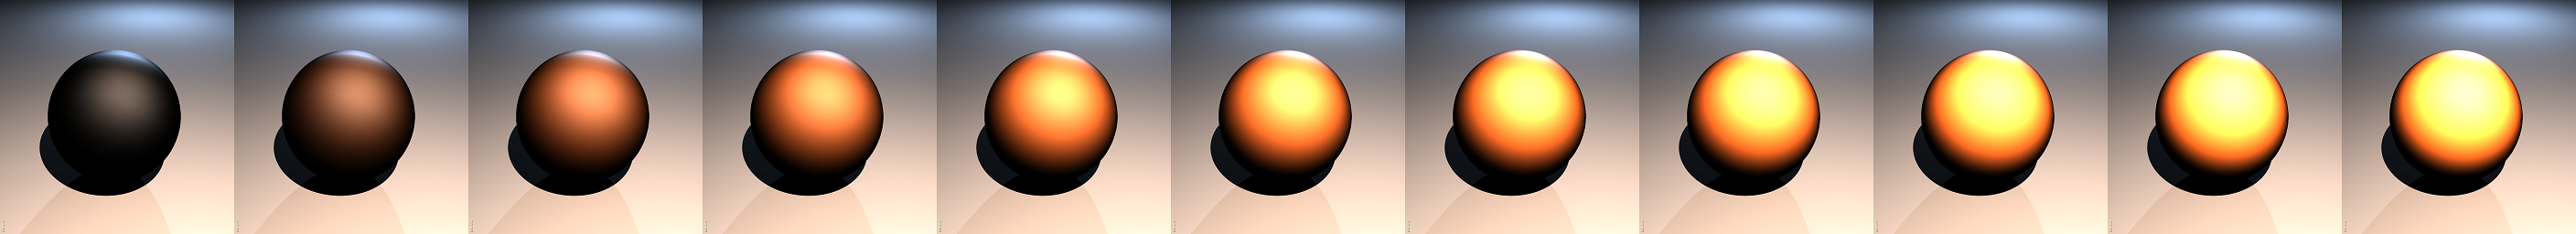
\includegraphics[width=\textwidth]{ashdiffcomplete.png}
\caption{Parameter $\rho_d$ from $0.0$ to $1.0$}
\end{figure}

\begin{figure}[H]

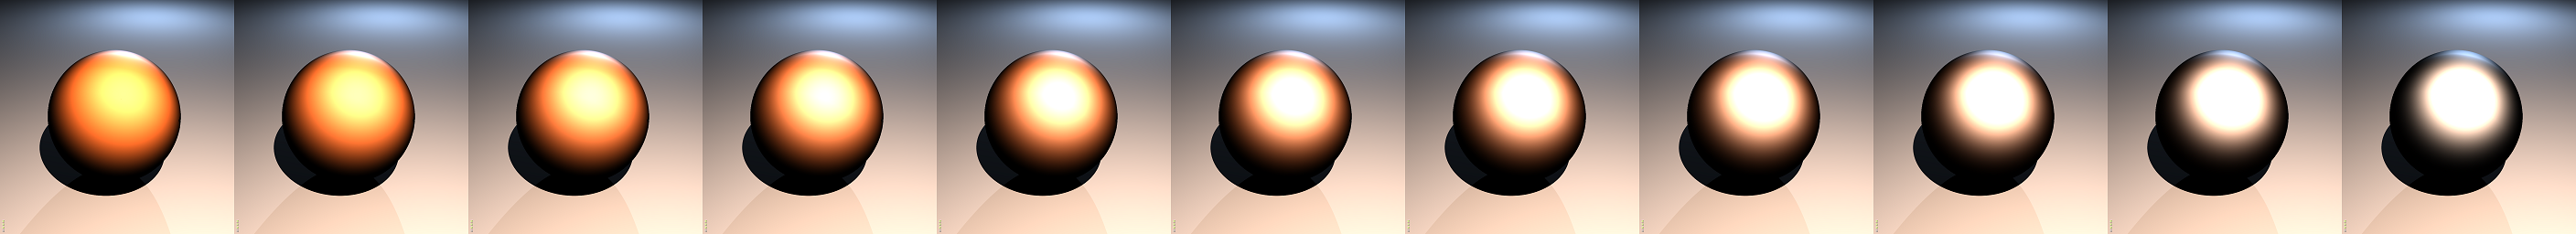
\includegraphics[width=\textwidth]{ashspeccomplete.png}
\caption{Parameter $\rho_s$ from $0.0$ to $1.0$}
\end{figure}

\begin{figure}[H]

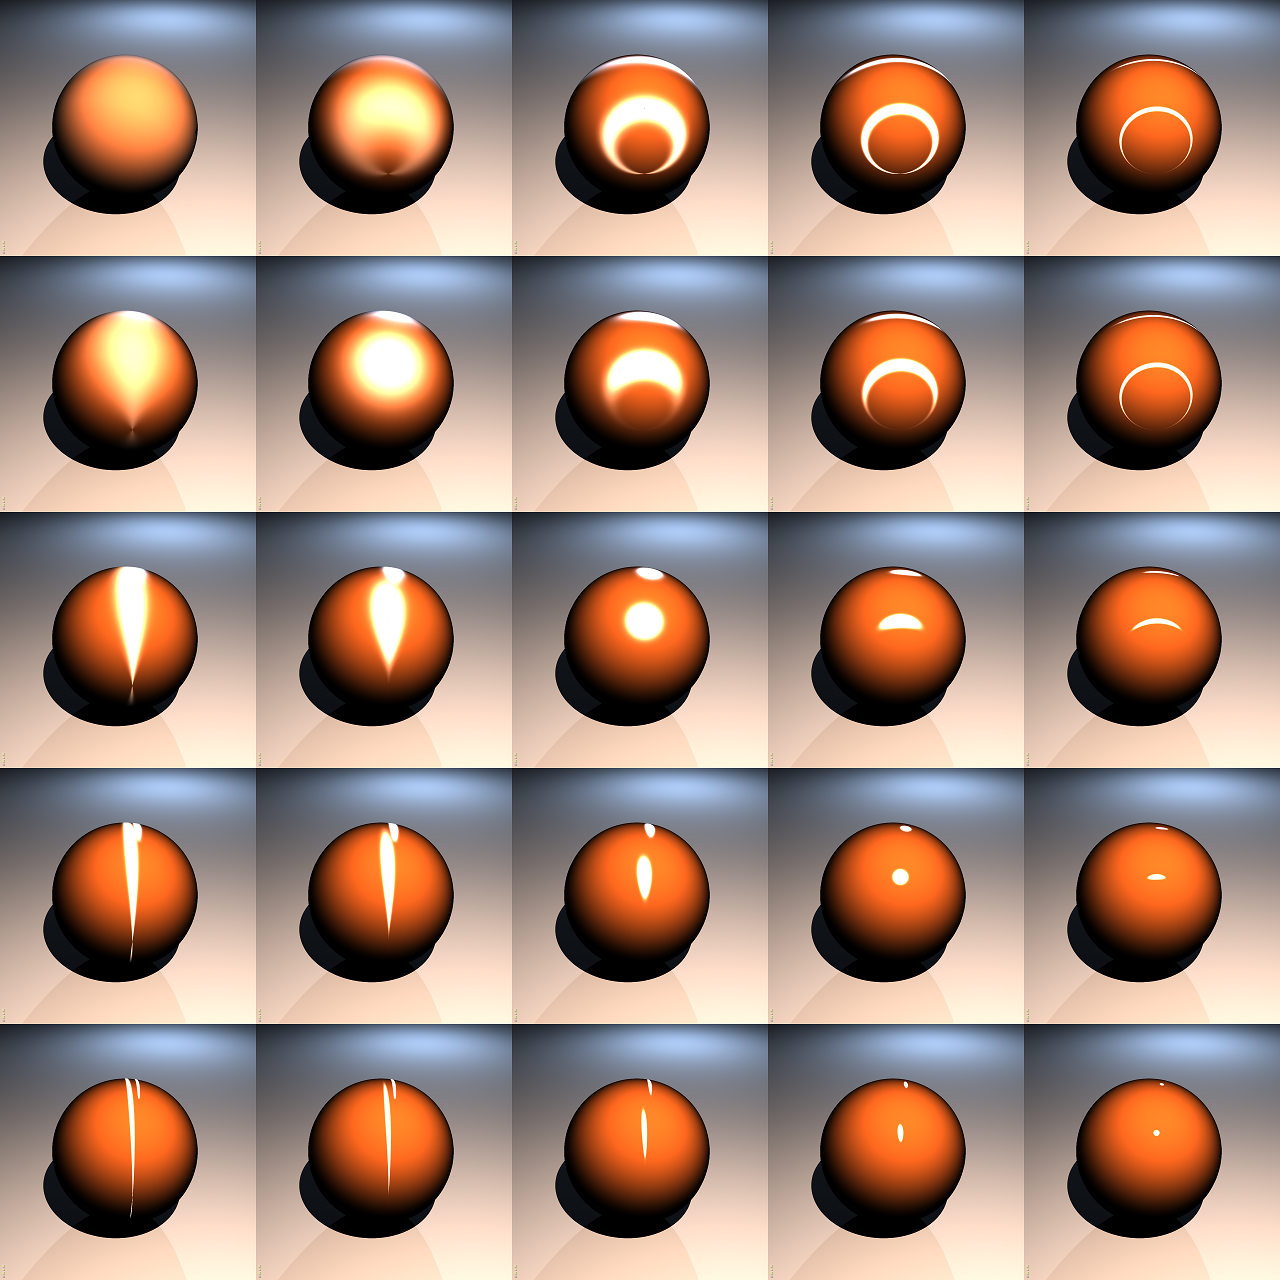
\includegraphics[width=\textwidth]{ashuvcomplete.png}
\caption{Parameter $n_u$, $n_v$ from $1$ to $10000$}
\end{figure}


\newpage
\subsection{Glass}

Glass is a dielectric material and can be described by a Dirac delta in the BSDF (bi-directional scattering distribution function). In fact, not even the same rendering equation can be used.
For Glass the following equation was used:

\begin{equation}
L_o(x,\vec{\omega_o})= \delta \cdot L_i(x,\vec{\omega_r}) + (1-\delta) L_i(x,\vec{\omega_t})
\end{equation}

\begin{table}[H]
\begin{tabular}{| c | l |}
\hline
$\delta$ & reflectivity of a dieletric\\ \hline
$\vec{\omega_r}$ & reflected view direction\\ \hline
$\vec{\omega_t}$ & transmitted view direction\\ \hline
\end{tabular}
\end{table}

A nice way to calculate $\delta$ is to use Schlick's Approximation \cite{Sch94}:
\begin{equation}
\delta(\theta) = \delta_0 + (1-\delta_0)(1-cos\theta)^5
\end{equation}
where:
\begin{equation}
\delta_0 = \left(\frac{n_t-1}{n_t+1}\right)^2
\end{equation}

\begin{table}[H]
\begin{tabular}{| c | l |}
\hline
$n_t$ & Parameter : refractive index of the surface\\ \hline
\end{tabular}
\end{table}


\begin{figure}[H]
\caption{Parameter $n_t$ from $1.0$ to $2.0$}
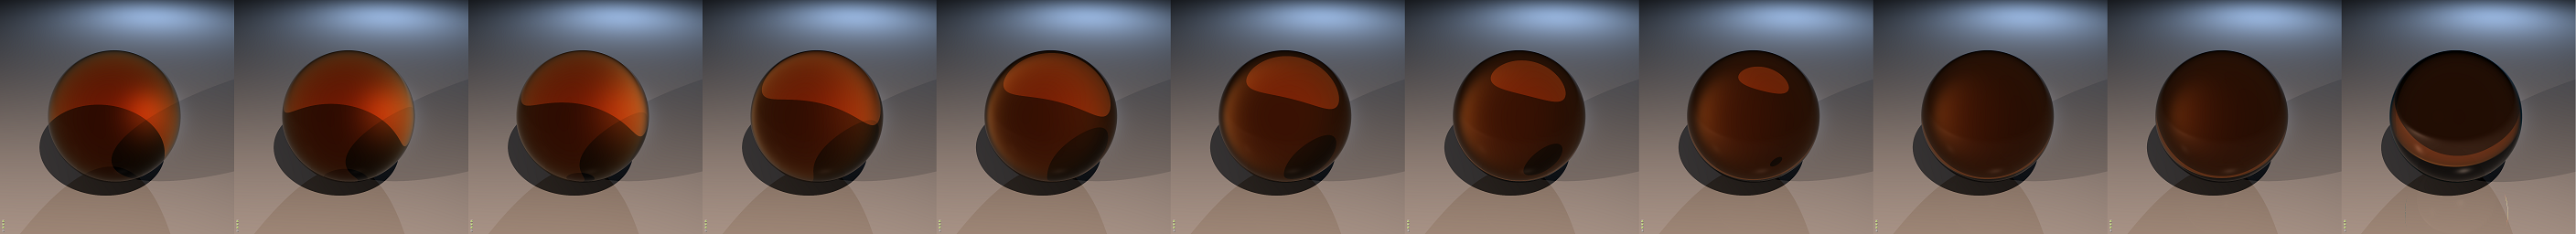
\includegraphics[width=\textwidth]{glasscomplete.png}
\end{figure}

\newpage
\section{Results}
In this section we will present some scenes we played with using our ray tracer

At first we compare it with ground truth, a ray tracer used in our "Computer Graphics I" class:
\begin{figure}[H]
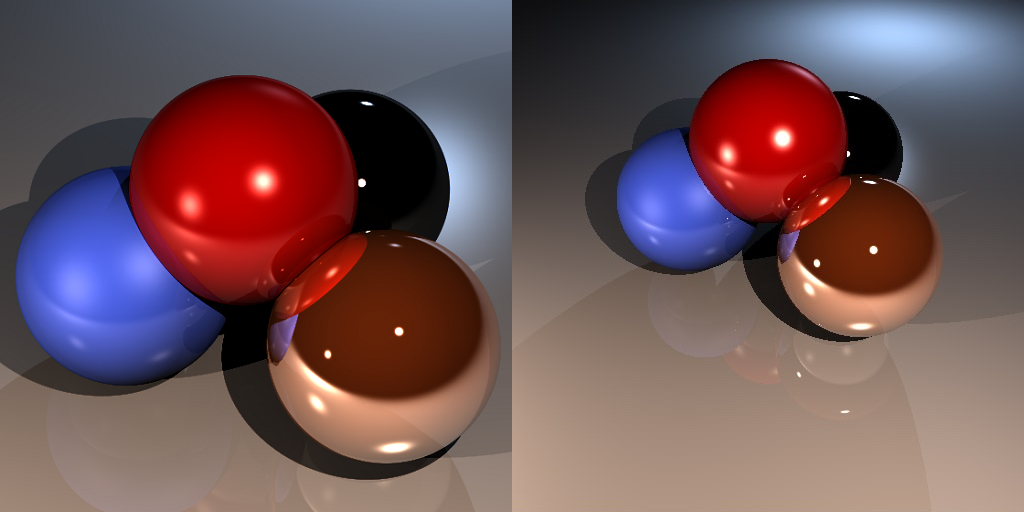
\includegraphics[width=\textwidth]{cgcomparison.png}

\caption{Left: Our Ray Tracer, Right: CG Ray Tracer}
\end{figure}

Everything seems very similar except the specular higlight on the surface of the red sphere. 

\begin{figure}[H]

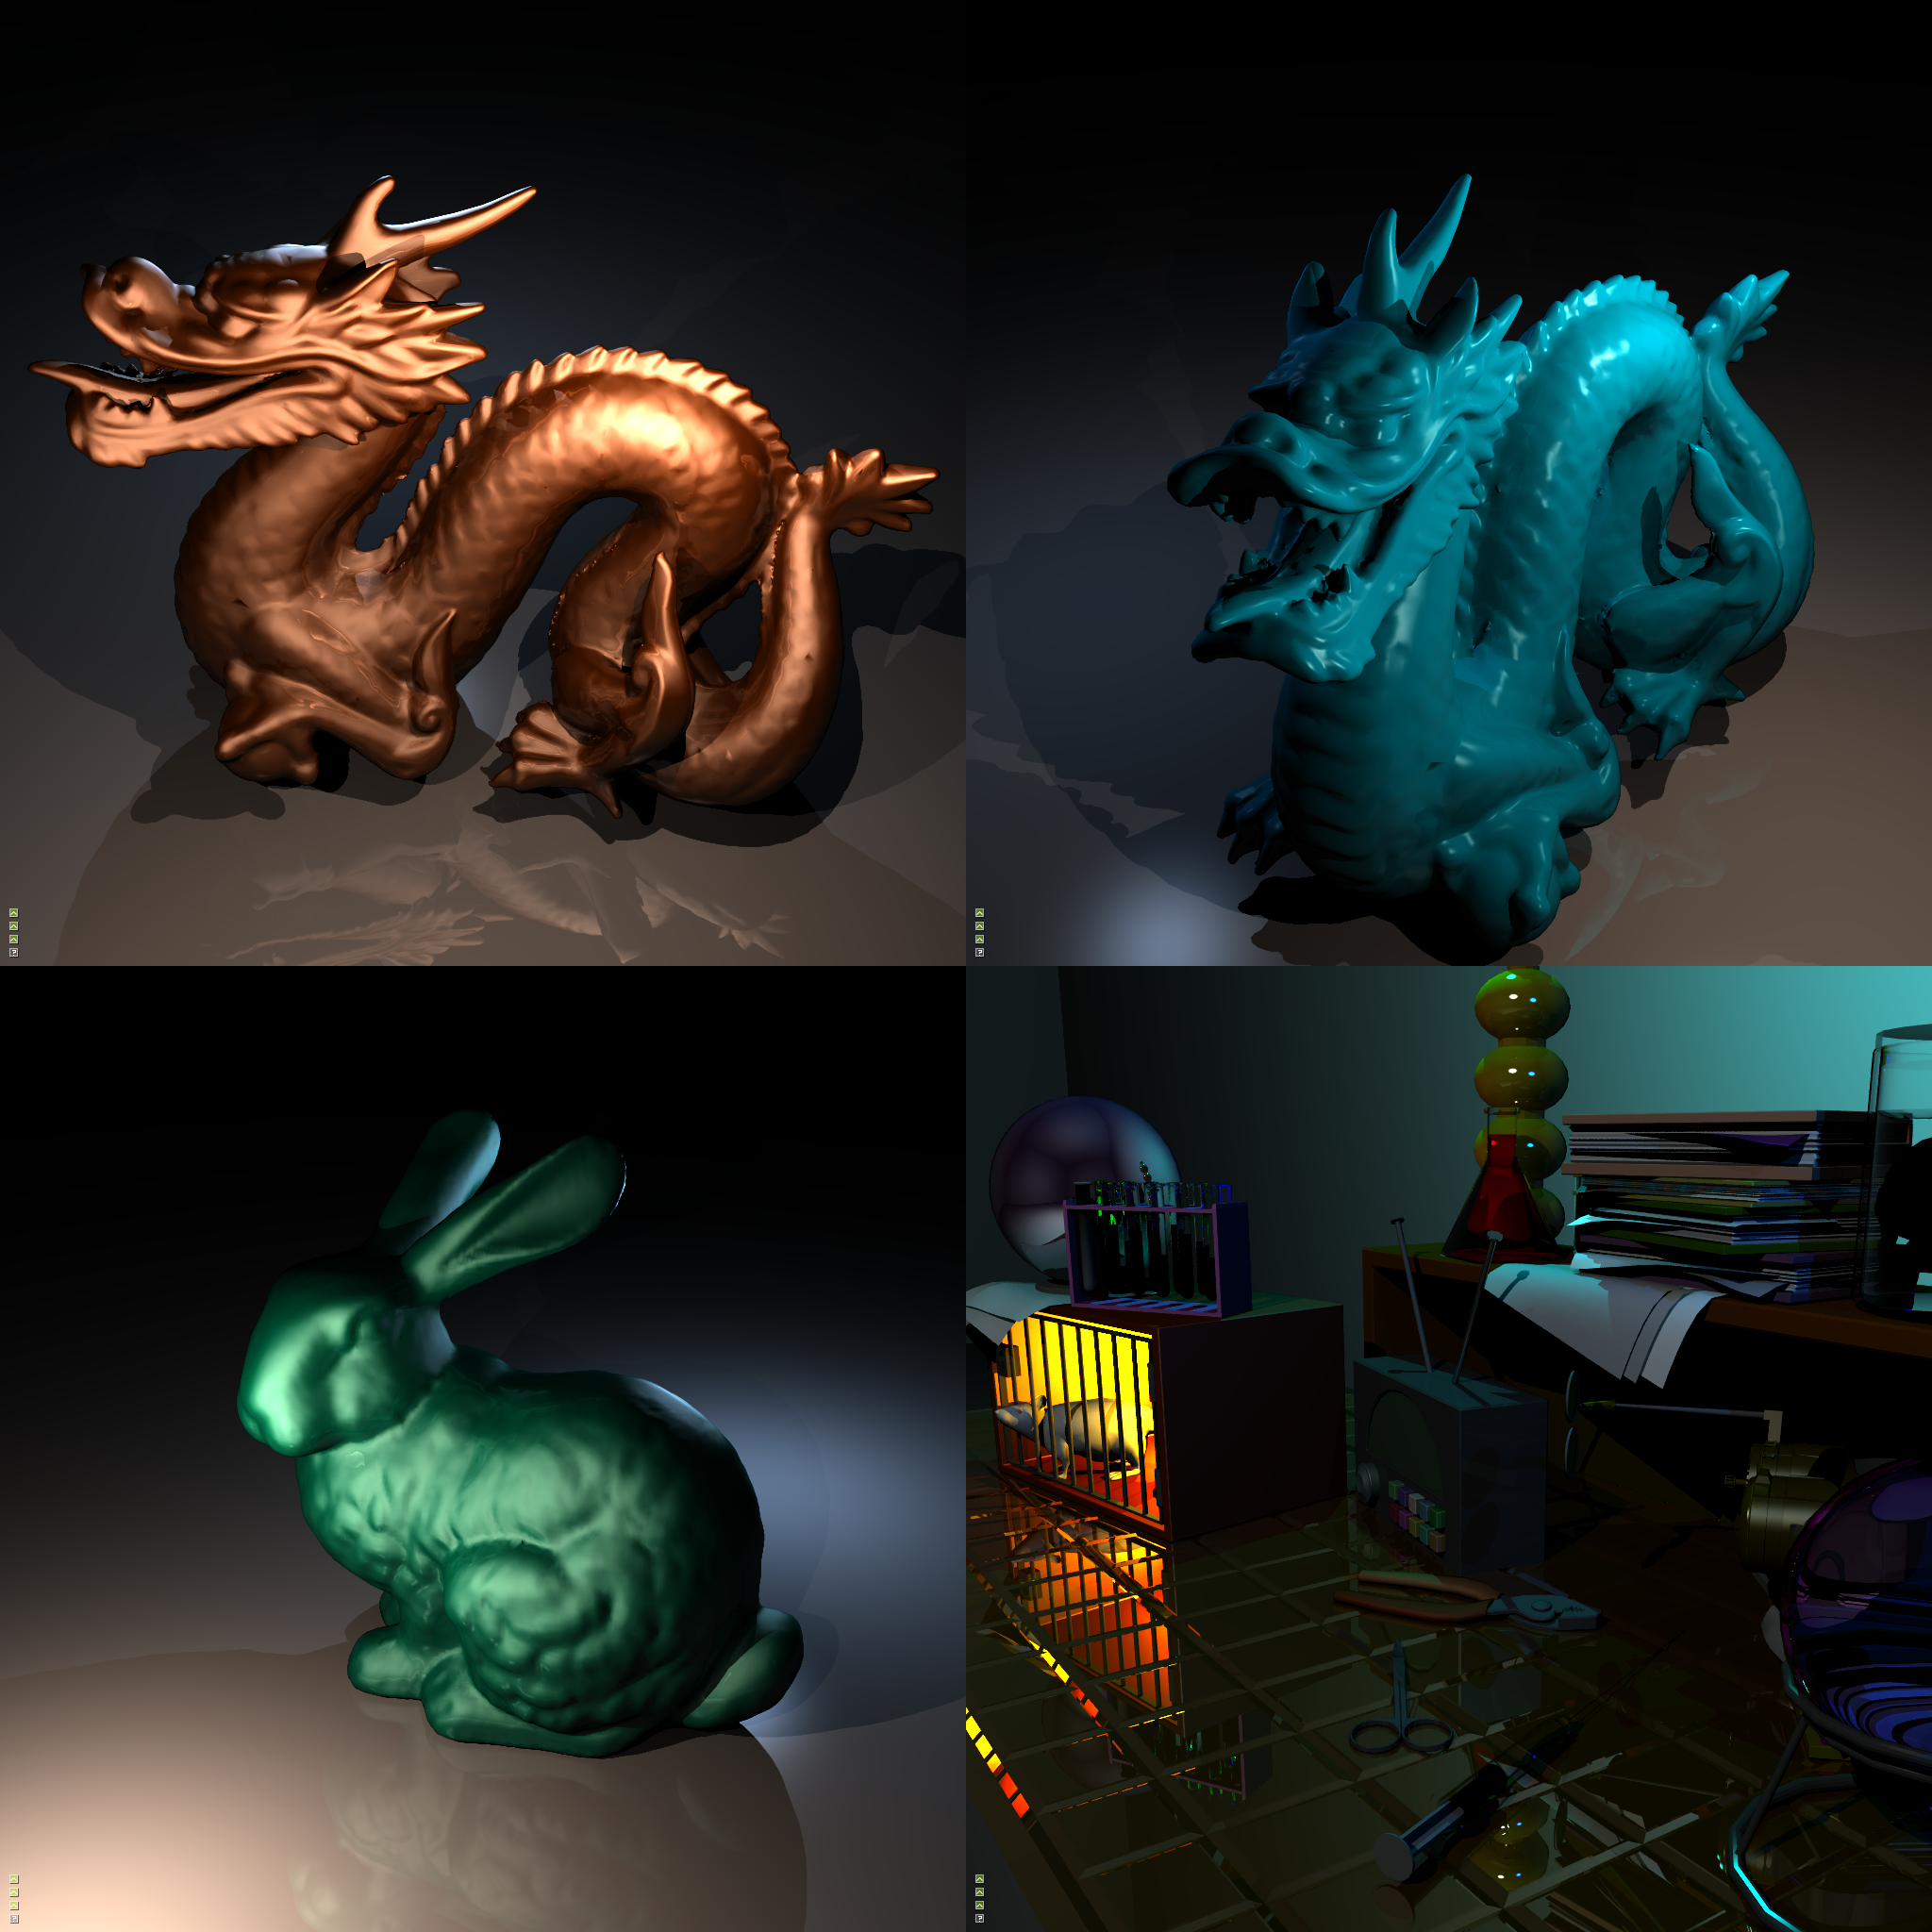
\includegraphics[width=\textwidth]{results.png}
\caption{From Upper Left to Lower Right: Copper Dragon(55fps) \cite{SU}, Blue Plastic Dragon(58fps), Yade Bunny(40fps) \cite{SU}, Mad Science(3fps) \cite{LC}}
\end{figure}

In the last Scene about 250 objects are rendered. Note that especially reflective and refractive materials are expensive in calculation. Unfortunately our glass material is not perfect which results in some artefacts on the surface. Intersection between models increase this effect.



\newpage
\section{Future Work}
In this section we will mention our future plans with this project as there are lots of interesting features, effects and enhancements to add to our current version of this project.

\begin{description}
\item[refactor material system:] At this point of time our used material system is very slow and uncomfortable to expand. As there will be more and more materials it is one of our favourite tasks to accomplish.

\item[fix glass:] As mentioned in Results there are still some bugs when using glass. These need to be fixed.

\item[add materials:]Especially the so called Disney-Principled BRDF is one we are looking for. Combining several other approaches to one intuitive, easy to use function, we are looking forward to implement this in our project.

\item[add textures:]Materials are a lot of fun, but at some point of capturing images they do not add enough details. Implementing the use of textures will fill this gap.

\item[use different lightsources:]By using other light sources than point lights, one is able to achieve great visual effects like soft shadowing. One step further, after sampling different area light sources, would be the use of environmental maps.

\item[load scene objects in groups:] By now every single object is loaded as one object as has to handled as this. The right parsing and grouping of objects will allow us greater and by far easier control of the scene.

\item[several lens effects:]Lens effects like depth of field or glare lens effects add interesting and good looking details to the scene.

\item[path tracing:]To reach the next step of realism in rendering , path tracing is inevitable.

\item[photon mapping:]Just like path tracing photon mapping has a great impact on the resulting image , especially when materials like glass are used.

\end{description}

\newpage
\addcontentsline{toc}{section}{References}
\bibliography{bericht}
\bibliographystyle{alpha}
\end{document}